\section{Circuits} 
%^
\begin{wrapfigure}[11]{R}{0.5\textwidth}
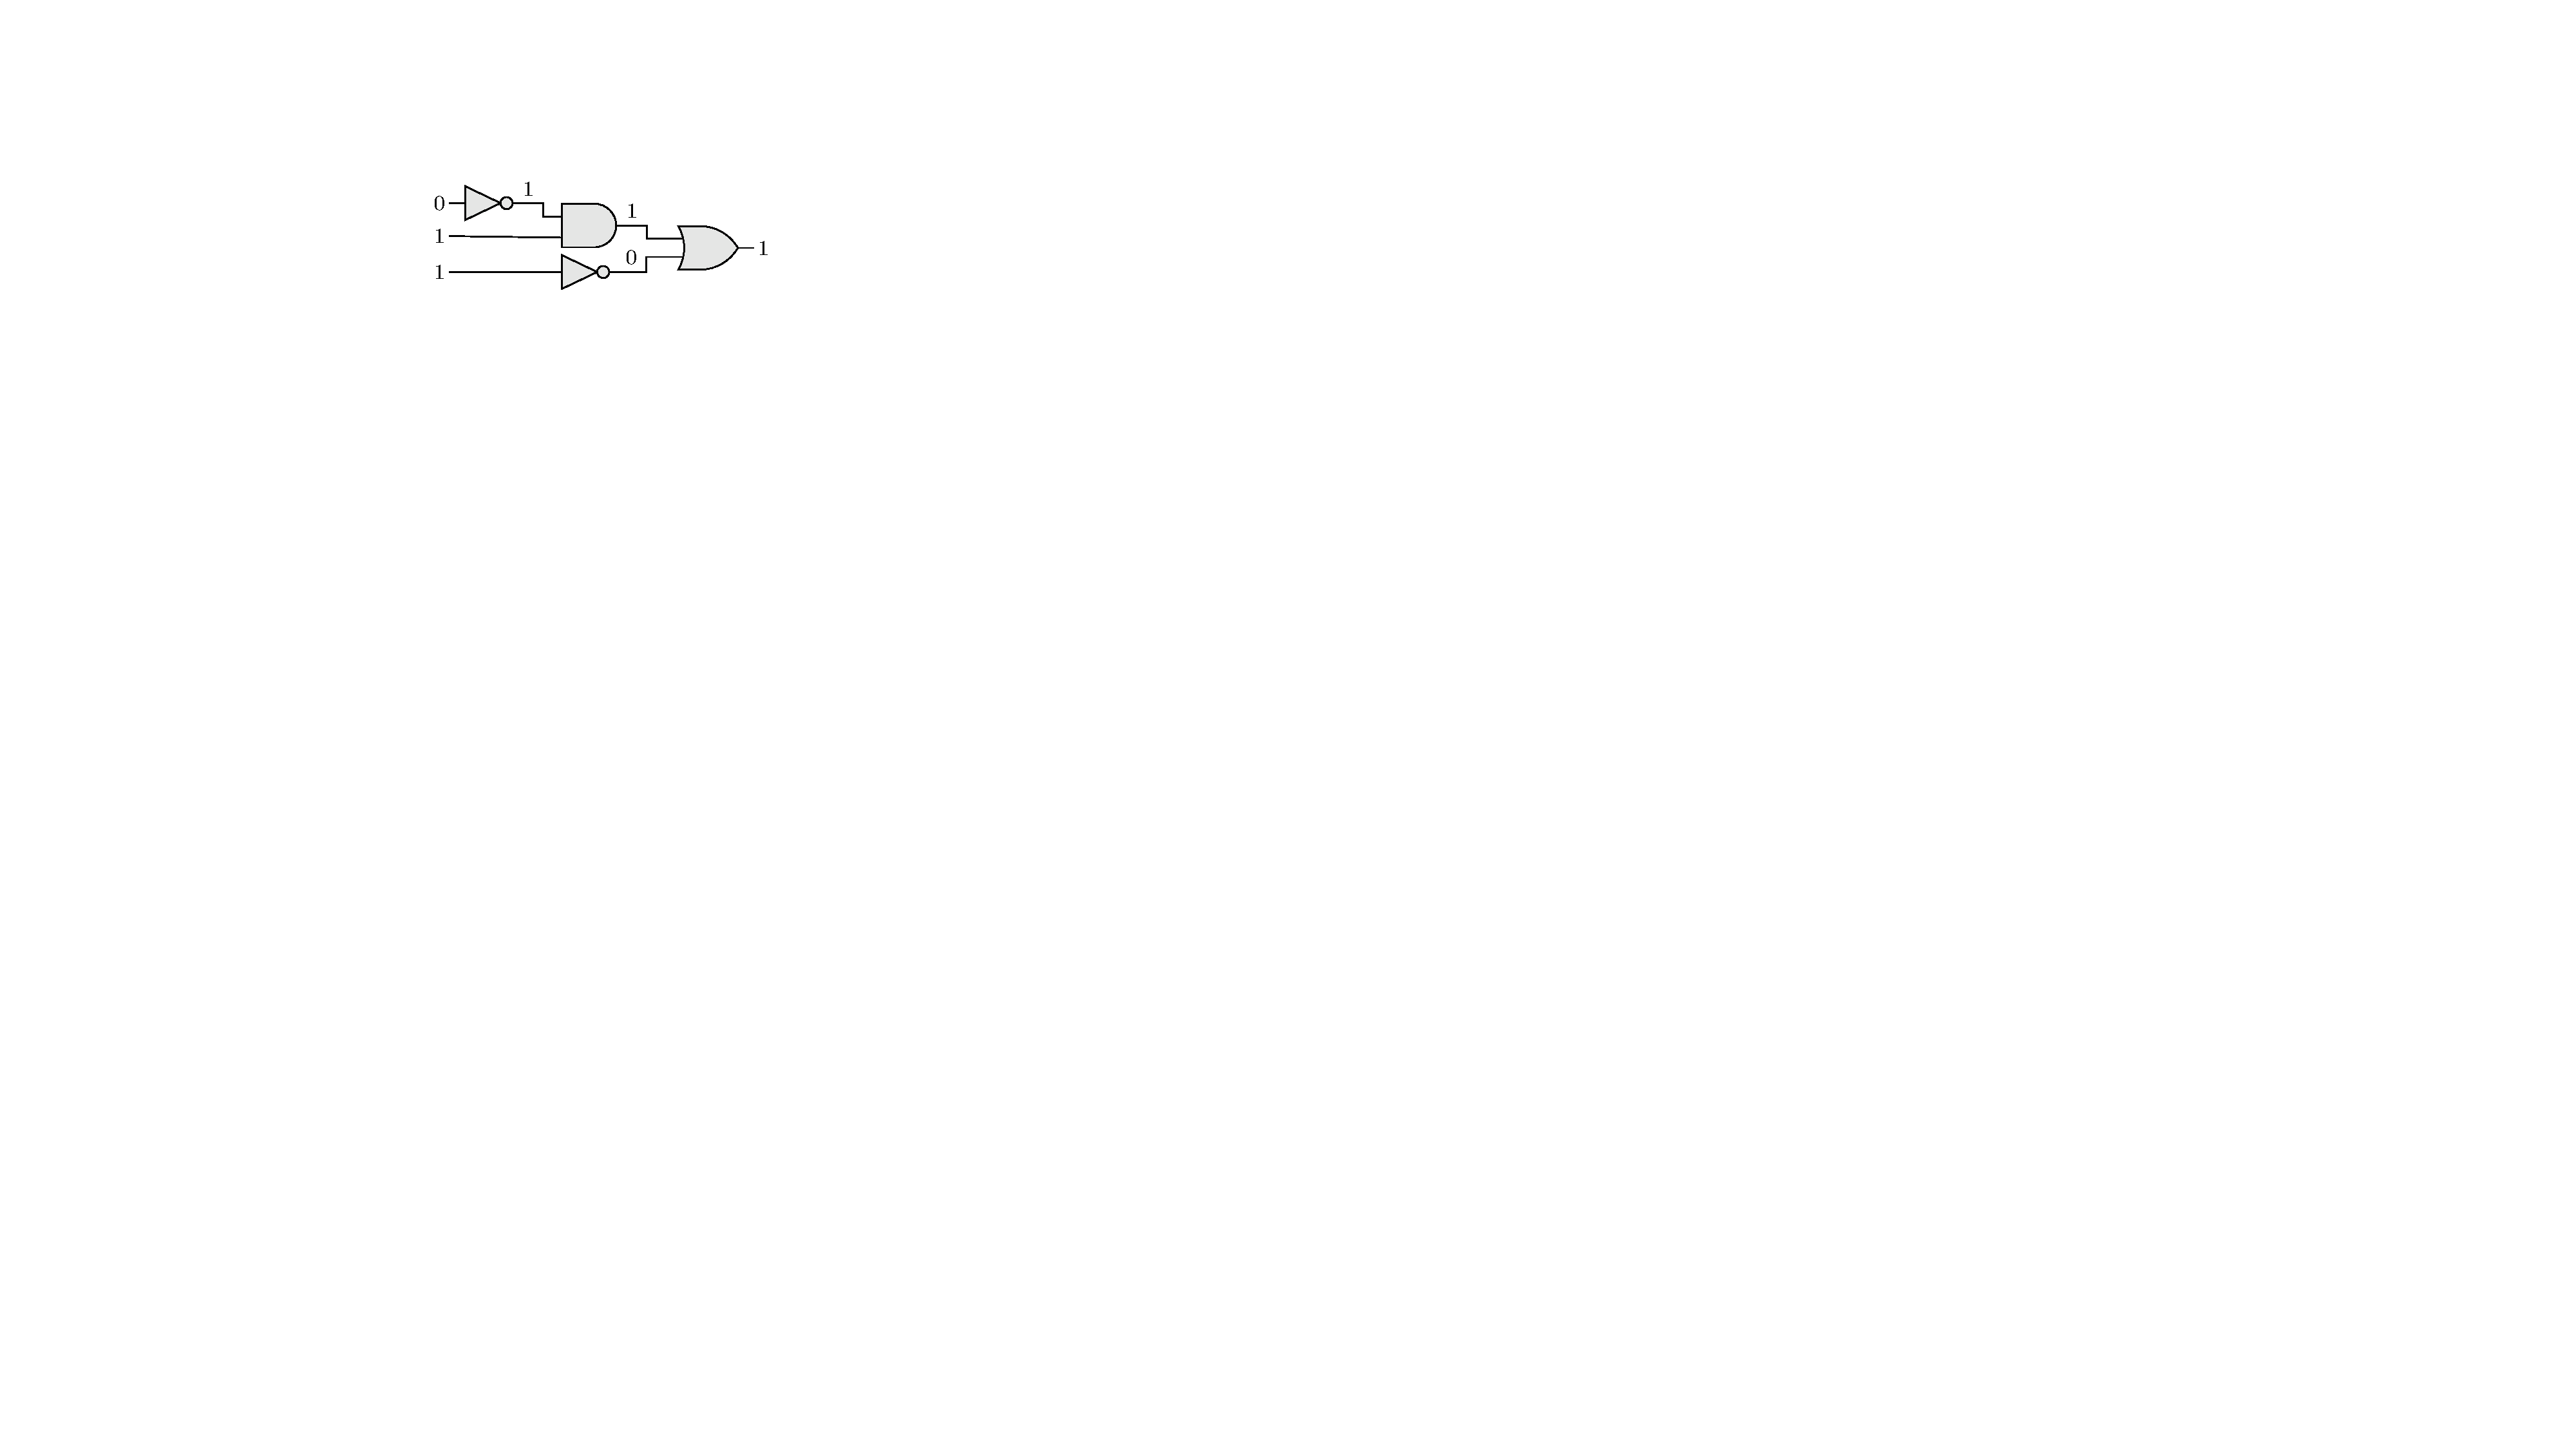
\includegraphics[width=0.48\textwidth]{Figures/HWCircuits/DigitalCircuit} 
\caption{A classical combinatorial circuit}
\label{classicalcirc:fig}
\end{wrapfigure}
A classical combinatorial circuit consists of a set of gates and acts as a~Boolean function. It takes a sequence of bits as input and produces a~sequence of bits as output. There are also internal bits that represent the connections between gates. In \cref{classicalcirc:fig}, the circuit has three input bits, one output bit, and three internal bits.
%
\begin{wrapfigure}{r}{0.5\textwidth}
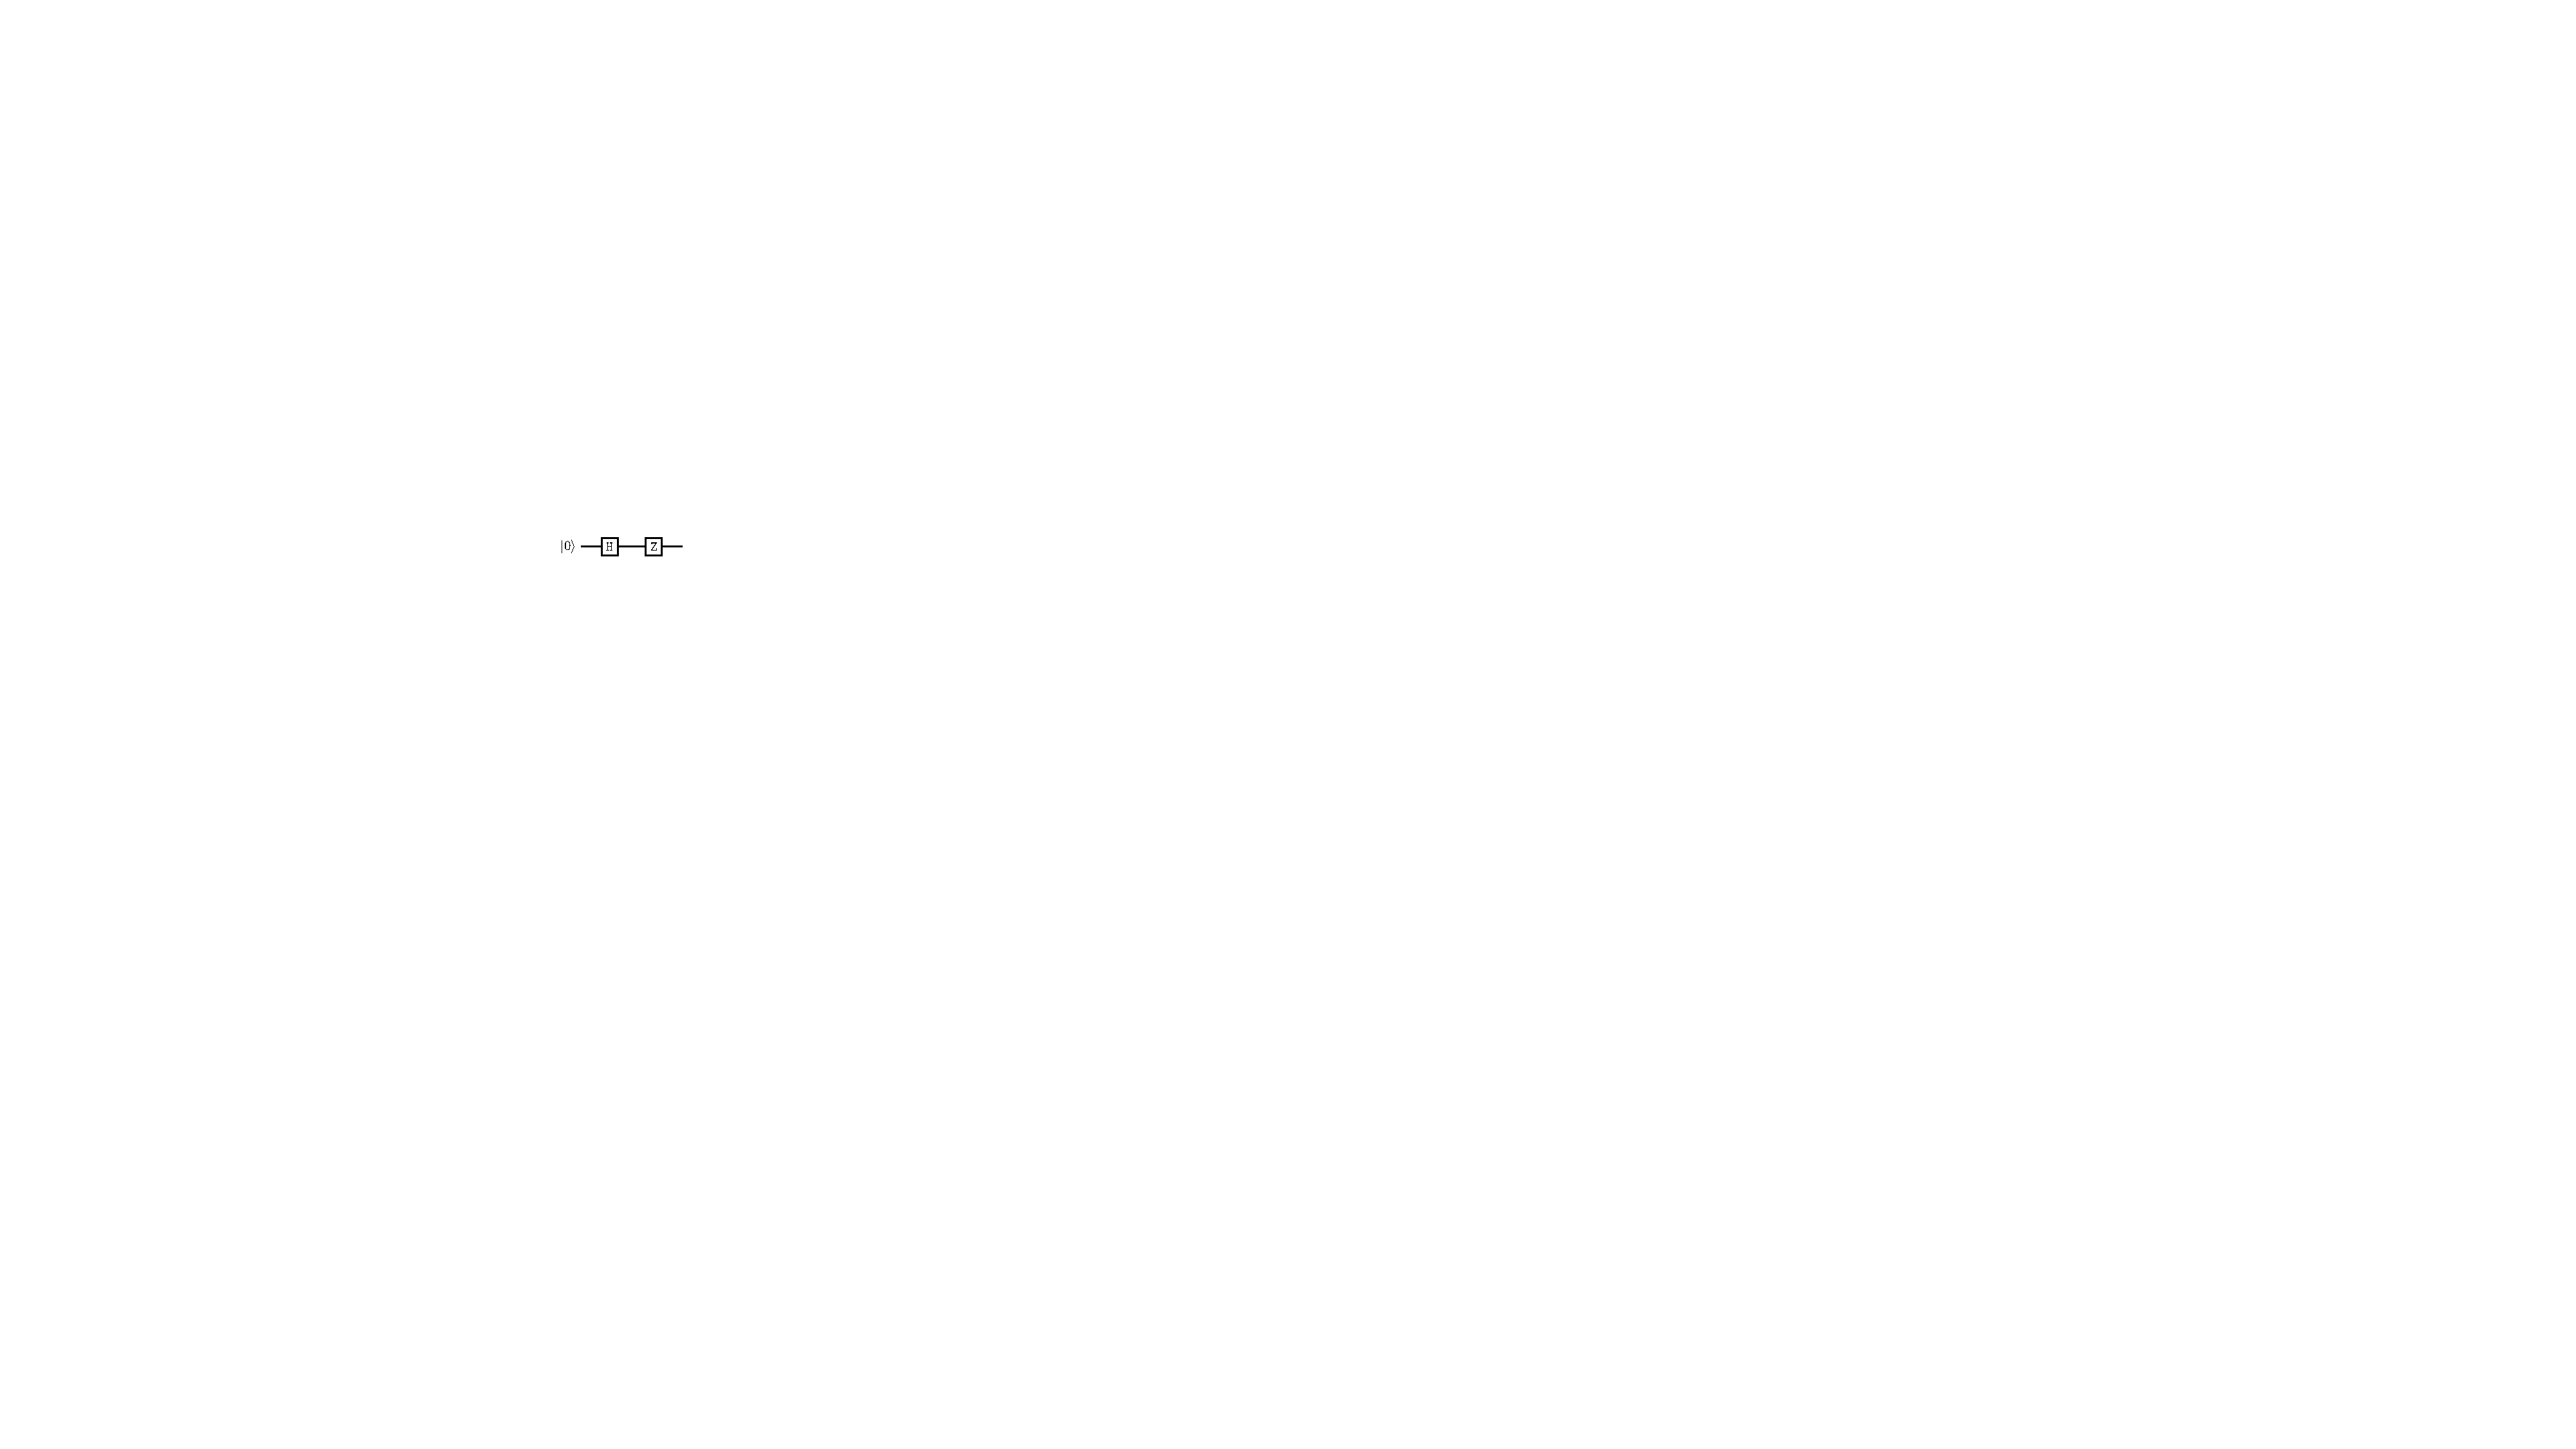
\includegraphics[width=0.48\textwidth]{Figures/Circuits/HZ} 
\caption{A simple quantum circuit.}
\label{HZ:fig}
\end{wrapfigure}
%
\cref{HZ:fig} shows a quantum circuit consisting of an $\hgate$ followed by a $\zpgate$ gate.

%^

We start with a qubit in a superposition state created using a Hadamard gate, and then apply a $\zpgate$ gate to it.
%
Here is a step-by-step description of the circuit behavior when the starting qubit is $\ketof0$.
%
\begin{enumerate}
\item Start in $\ketof0 = [1 \;\; 0]^T$
\item Apply the Hadamard gate: 
$H\ketof0 = \frac{1}{\sqrt{2}}(\ketof0 + \ketof1)$
%
Now the qubit is in an equal superposition.
\item Apply the $\zpgate$ gate: 
$\zpgate\left(\frac{1}{\sqrt{2}}(\ketof0 + \ketof1)\right) = \frac{1}{\sqrt{2}}(\ketof0 - \ketof1)$.
%
The $\ketof1$ term’s sign flips—this is phase inversion.
\end{enumerate}

Intuitively, the Hadamard spreads the probability amplitude across both states.
%
The $\zpgate$ keeps the probability unchanged (as it only affects the phase), but introduces a phase shift to $\ketof1$, which is crucial in interference patterns for quantum algorithms.

%^

\begin{figure}[ht] 
    \centering
    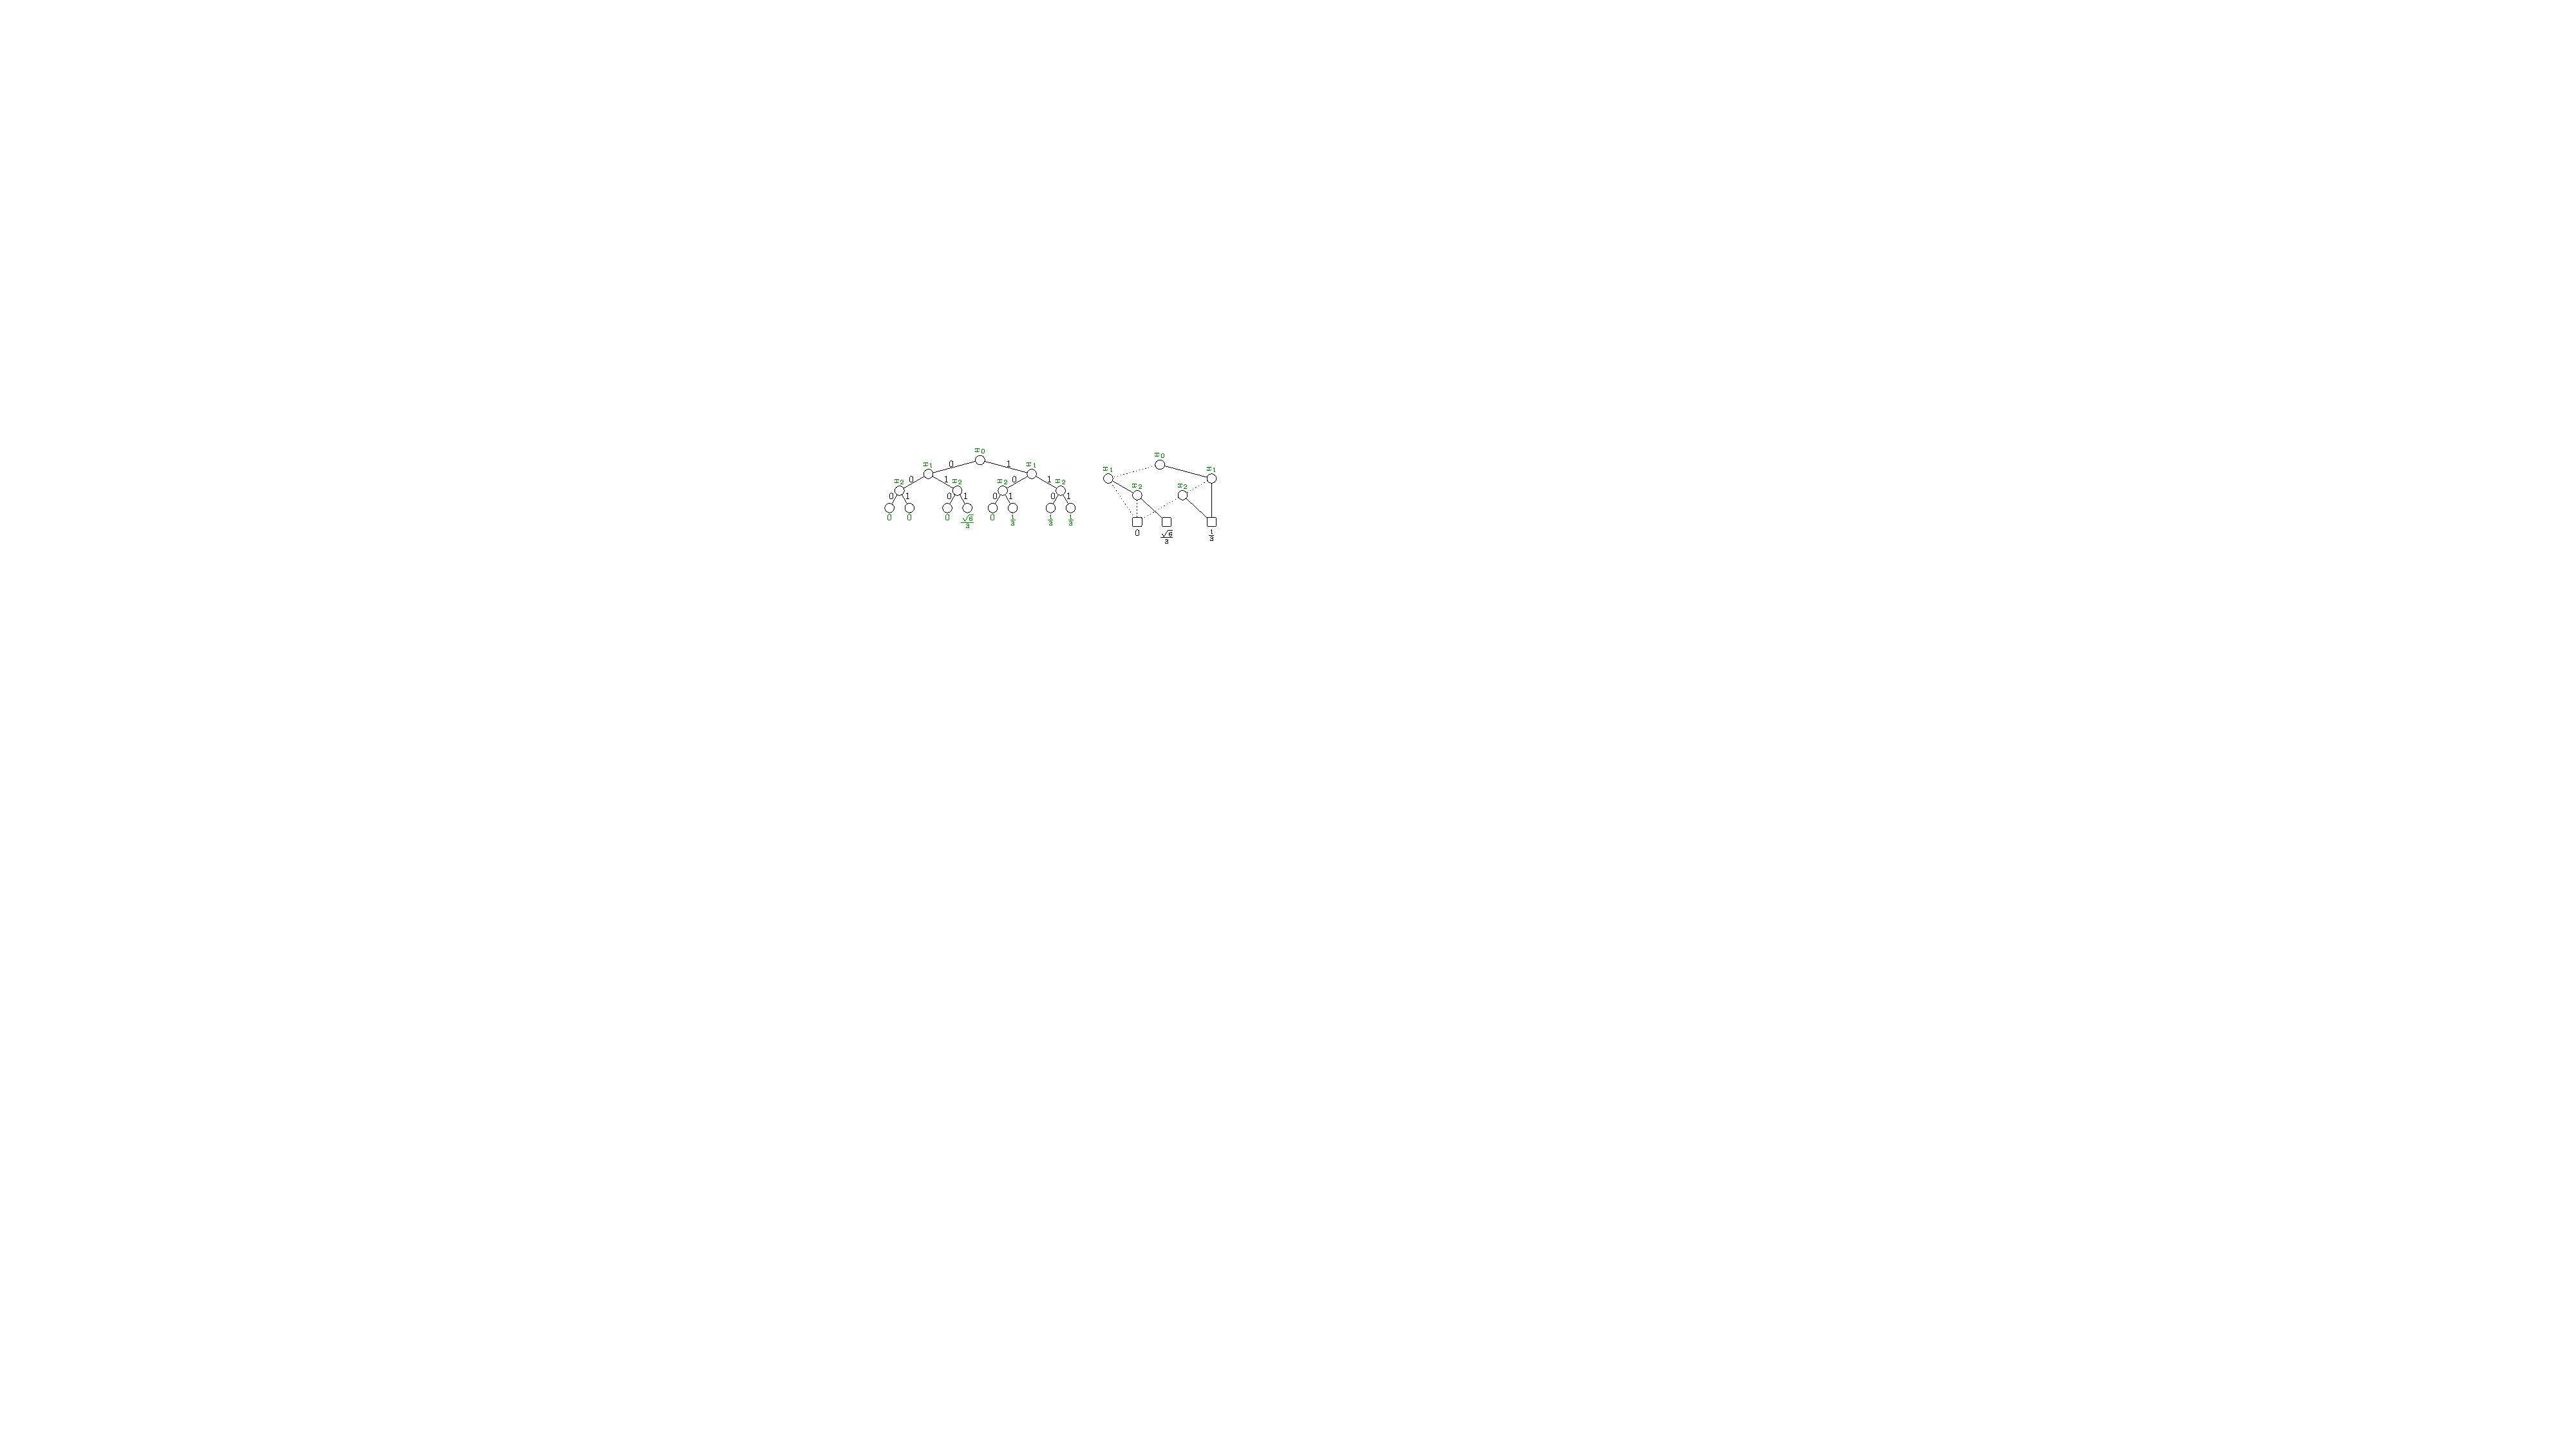
\includegraphics[scale=1.2]{Figures/BDDs/BDDs} 
    \caption{The BDD representation of a quantum state.}
    \label{BDD:fig}
\end{figure}

%

\section{Program Verification and Hoare Logic}
%
Next, we turn our attention to the verification problem and consider the classical framework of \emph{Hoare logic}.  
%
This formal verification method was initiated by  Floyd~\cite{Flo67a} and further developed by Hoare~\cite{DBLP:journals/cacm/Hoare69}.  
%
The core concept of this logic is the \emph{Hoare triple}, written in the form:
\[
\{P\}\, C\, \{Q\}
\]
where $P$ is the \emph{precondition}, $Q$ is the \emph{postcondition}, and $C$ is a program.  
%
A Hoare triple is said to be \emph{valid} if the following condition holds:
If the program $C$ is executed from an initial state $\sigma$ satisfying the precondition $P$ (i.e., $\sigma \models P$), then the execution terminates in a final state satisfying the postcondition $Q$.
%
The initial obstacle in the application of the framework was the state space explosion problem that occurred due to the large size of the state space of $C$.
%
A fundamental breakthrough in the verification of conventional computer systems was the invention of efficient data structures to represent sets of states.
%^
A case in point is the classical BDD (Binary Decision Diagram) data structure.
%
\cref{BDD:fig} depicts a BDD representation of a quantum state.

In this paper, we take $C$ to be a quantum circuit.
%
%
The main challenge in using BDDs in quantum circuits is the fact that a BDD represents a single state.
%
In conventional circuits, a BDD represents a (large) set of states.
%
Thus, we need a framework in which we can handle sets of BDDs.
%
Given that we represent quantum states by trees, a natural choice is to use tree automata to represent sets of quantum states.
%^
\begin{figure}[ht] 
    \centering
    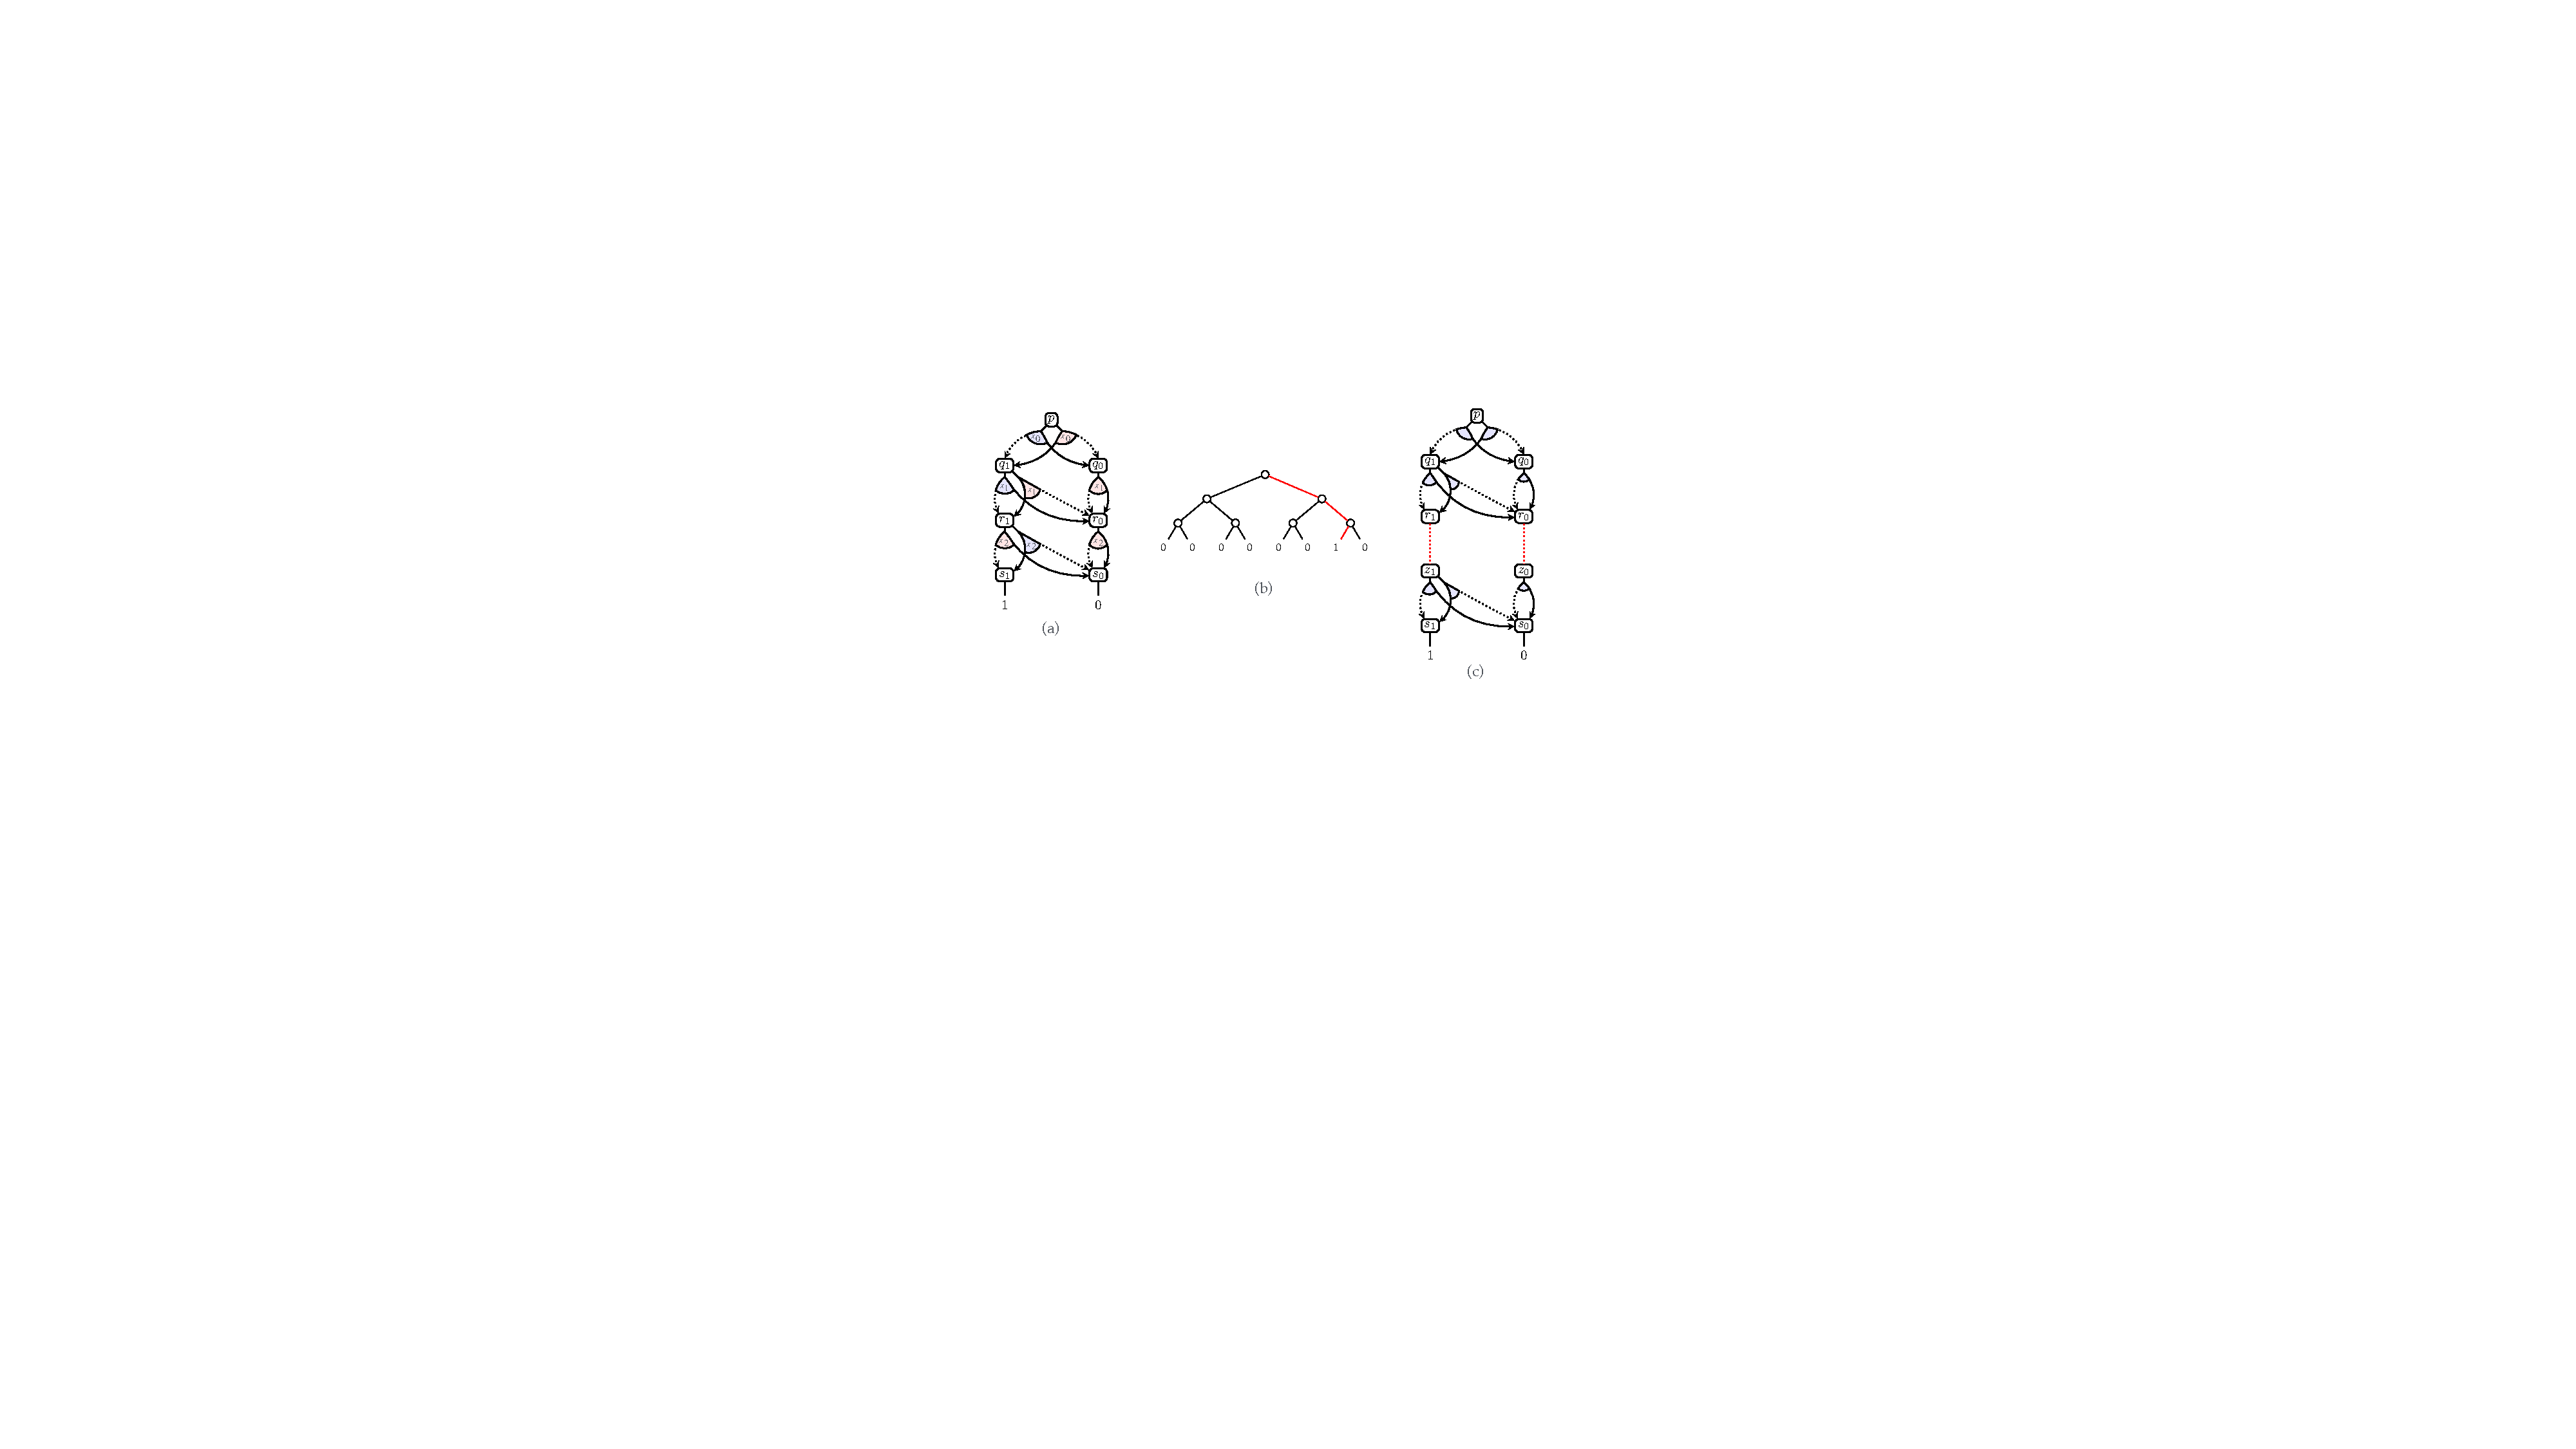
\includegraphics[scale=0.8]{Figures/Automata/aut3} 
    \caption{(a)~A tree automaton for generating all basis states of $3$ qubits.
      The dashed lines represent the left-hand child, and the solid lines represent the right-hand child.
      (b)~The tree corresponding to $[0\;0\;0\;0\;0\;0\;1\;0]^T$. The rules, shadowed in pink, in the automaton are those used to generate the tree.
      (c)~An automaton to generate all basis states of $n$ qubits.}
    \label{automata:fig}
\end{figure}
%
\cref{automata:fig}(a) gives a tree automaton for accepting all basis states of size three.
%
The set of rules is the following:
\[
\begin{array}{lll}
p \xrightarrow{x_0} (q_0, q_1) &
\;\;\;\;\;\; p \xrightarrow{x_0} (q_1, q_0) & \\
q_0 \xrightarrow{x_1} (r_0, r_0) &
\;\;\;\;\;\; q_1 \xrightarrow{x_1} (r_1, r_0) &
\;\;\;\;\;\; q_1 \xrightarrow{x_1} (r_0, r_1) \\
r_0 \xrightarrow{x_2} (s_0, s_0) &
\;\;\;\;\;\; r_1 \xrightarrow{x_2} (s_1, s_0) &
\;\;\;\;\;\; r_1 \xrightarrow{x_2} (s_0, s_1) \\
s_0 \xrightarrow{} 0 &
\;\;\;\;\;\; s_1 \xrightarrow{} 1
\end{array}
\]
%
Notice that we are characterizing $2^n$ basis states using only $3n+1$ transitions.
%
\begin{figure}
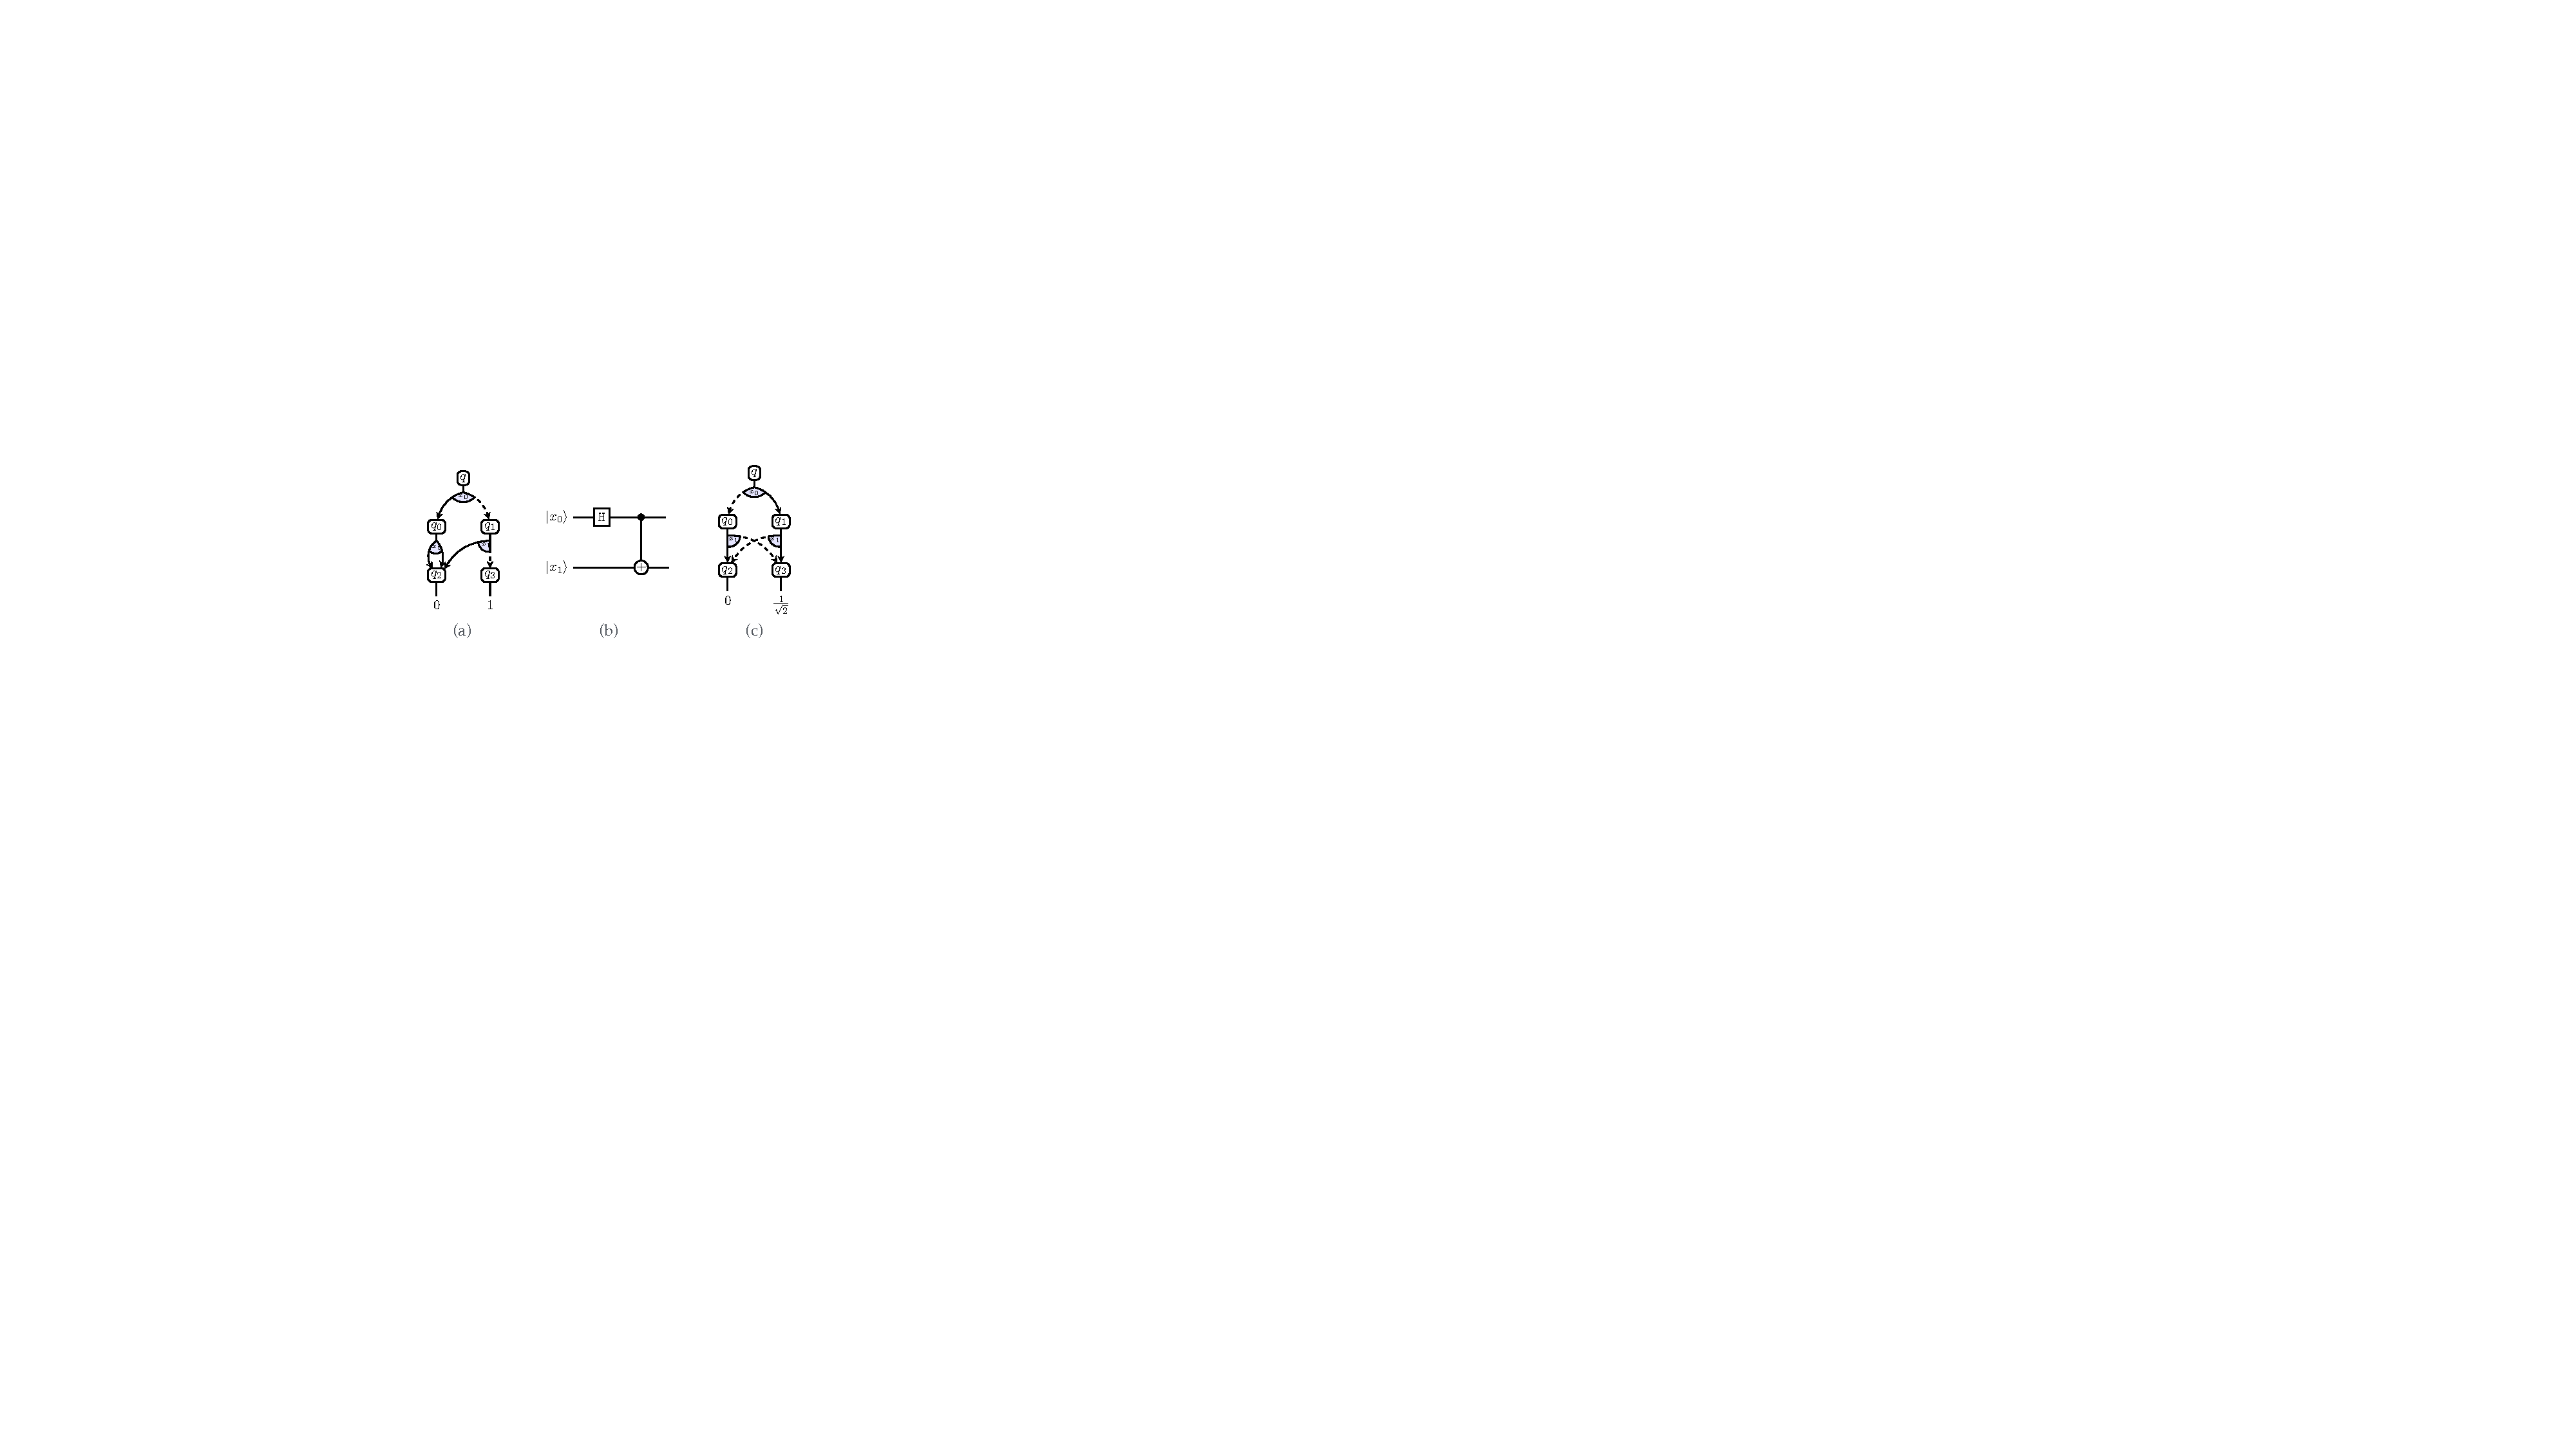
\includegraphics{Figures/Circuits/Bells}
\caption{The circuit for the Bell state.
  }
\label{Bells:fig}
\end{figure}
%
In our setting, a gate application corresponds to a tree transformation.
%
For a circuit consisting of a number of gates, we provide an algorithm that transforms a tree automaton describing a set of input states to a new automaton describing the set of output states.
%
We do this by constructing a sequence of automata that model the effects of each gate.
%
\cref{Bells:fig} gives a concrete example to demonstrate our approach.
Assume we want to design a circuit constructing the Bell state, i.e., a 2-qubit circuit converting a basis state $\ketof{00}$ to the maximally entangled state $\frac{1}{\sqrt{2}}(\ketof{00} + \ketof{11})$.
%
Given the automaton corresponding to the pre-condition (\cref{Bells:fig}(a)), we derive the automaton corresponding to the post-condition (\cref{Bells:fig}(c)).
%
In this case, both automata use $q$ as the root state and accept only one tree.
%
We can observe the correspondence between quantum states and tree automata by traversing their structures.

%
